%
% Prototype Formation
%

\subsection{Category Learning in Autism}
Prototype formation is invaluable for learning concepts and categories. A category prototype is a kind of representational average of the features of category members that have been seen. Some studies have suggested that, when learning a new concept or category, children with autism are less likely to form a prototype representation than typically developing children~\cite{KlingerLG:2001:Prototype,GastgebHZ:2009:Prototype}. Difficulty identifying an abstract prototype is argued to underly the generalization problems found in ASD.

Typically developing children exhibit a ``prototype effect'' when they are shown objects in a category and are then asked to categorize novel objects. This effect involves more reliably and/or more quickly identifying a prototype object as a member of a target category, in comparison to other test objects. Klinger \& Dawson~(2001) \nocite{KlingerLG:2001:Prototype} found that people with ASD do not exhibit the ``prototype effect''.

In the Klinger and Dawson (2001) experiment, paricipants viewed cartoon pictures of imaginary animals, with each animal belonging to one of a small set of fictional animal categories. The members of each category of animal varied in four features. For example, animals in the ``Mip'' category varied in the sizes of horns, wings, mouths, and feet. Each feature could take on one of five discrete values, ordered 1 to 5 (e.g., horns always were of one of five specific sizes). Thus, individual cartoons could be specified by four feature values (e.g., ``5115'' for largest horns, smallest wings, smallest mouth, and largest feet). Different animal categories had distinct sets of four features, as illustrated in Figure~\ref{prototype-categories}.

The children initially learned to classify a target category of animals (e.g., ``Mip'') in contrast to a single non-target category (e.g., ``Pev''). A member of the target category was first dislayed, and the target category name was provided (e.g., ``This is a Mip.''). Participants were then presented with a series of target and non-target stimuli, one at a time, and they were asked to identify the members of the target category. As is clear from Figure~\ref{prototype-categories}, this category learning task was easy, as different animal categories possessed different sets of features. Corrective feedback was provided after each response. During this learning process, the presented target category stimuli only used feature values 1, 2, 4, and 5, but never 3. (See Figure~\ref{mip-familiarization}.) Only a subset of the possible combinations of feature values appeared, but the average value used for each feature in the target category was 3, making the unobserved ``3333'' stimulus object the prototype for the category.

Immediately following this learning process, participants were tested for the ``prototype effect''. On each test trial, two animals from the target category were juxtaposed, and participants were asked to select one as the ``best'' category member (e.g., ``Which is the best Mip?''). The trials of interest involved pairing the prototype (``3333'') with either a previously viewed animal or one that was novel but was composed only of previously viewed feature values (e.g., ``1425''). Typically developing children chose the prototype at a rate significantly higher than chance ($79\%$). However, children with autism selected the prototype at a rate indistinguishable from chance ($54\%$).
% (See Figure~\ref{klinger_results}.)
Klinger and Dawson argued that these results demonstrated a lack of prototype formation in ASD.

\begin{figure}[ht]
\begin{center}
	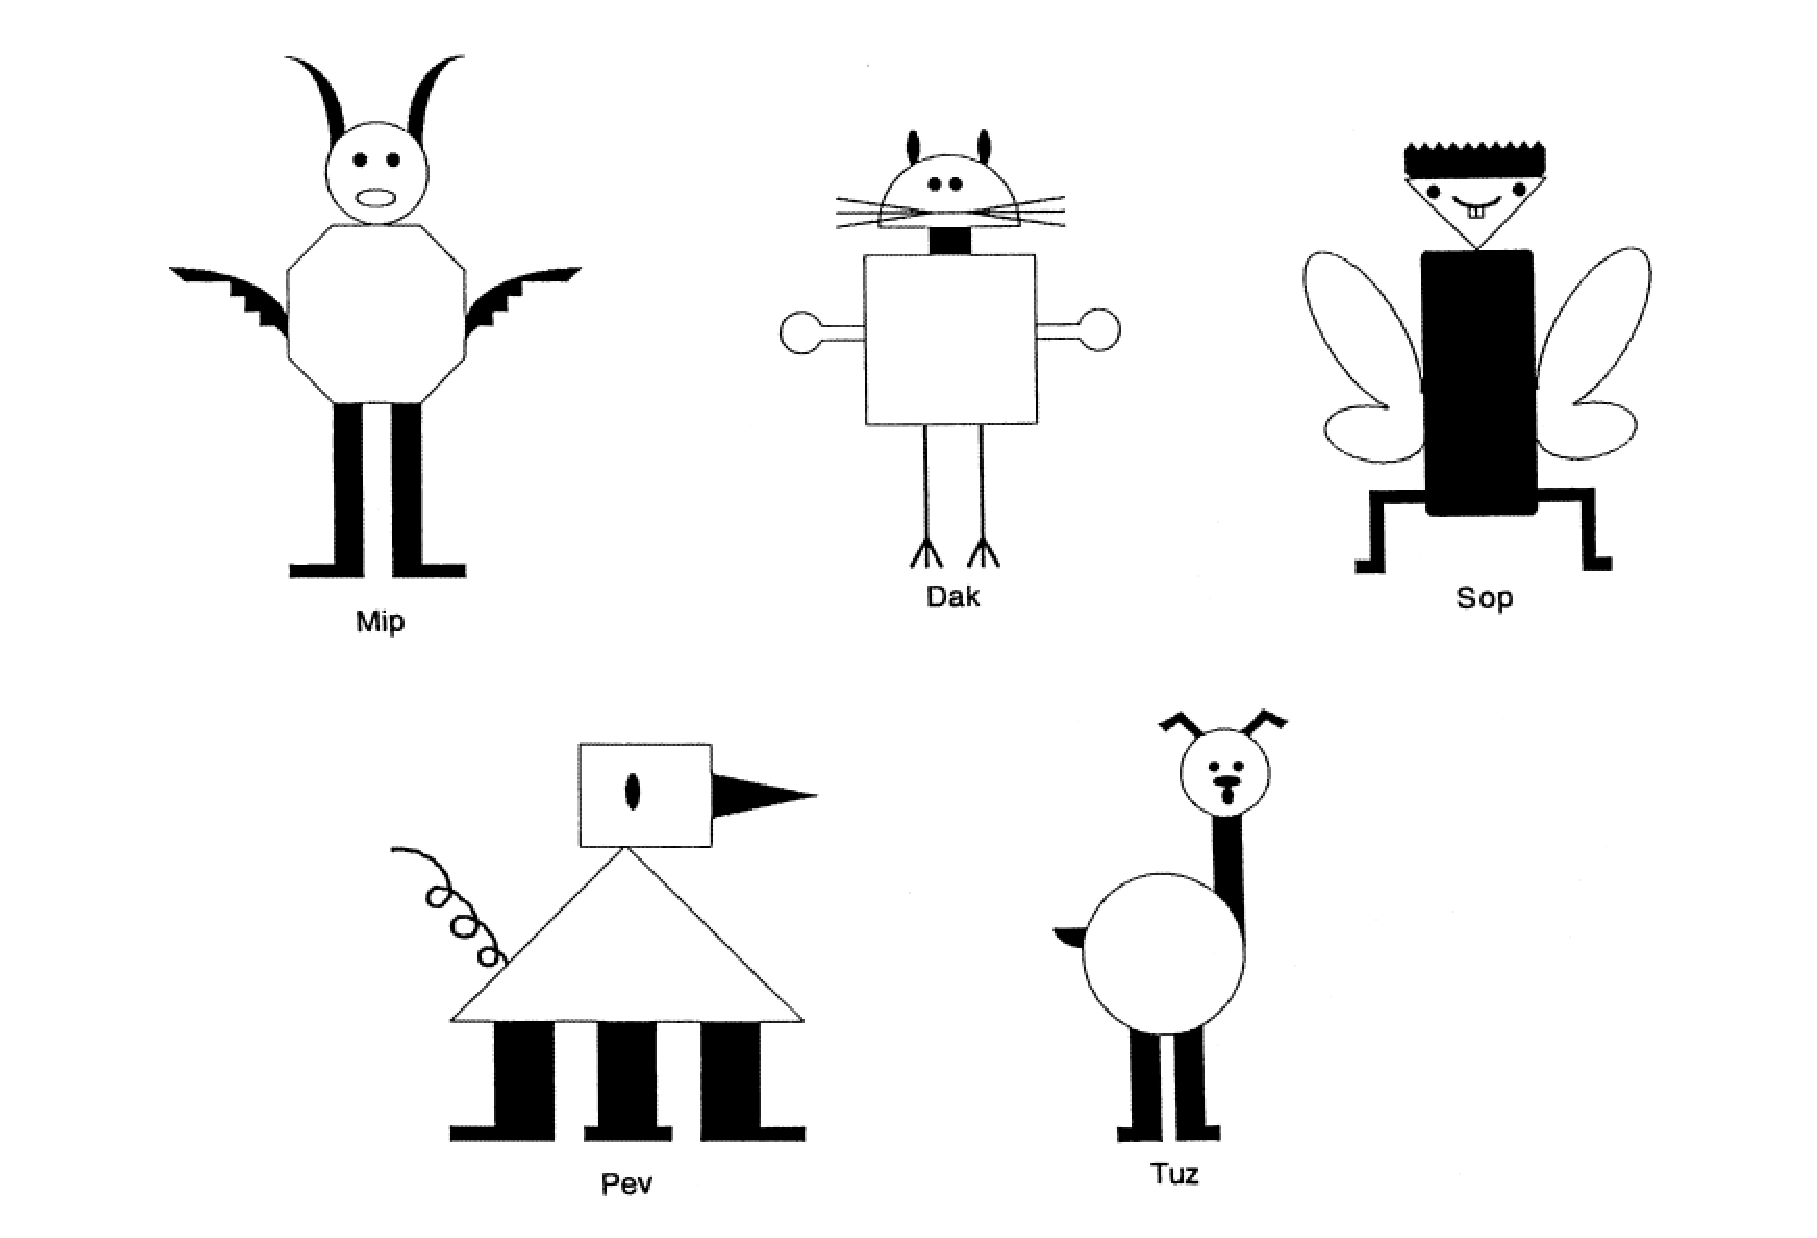
\includegraphics[width=75mm]{figures/prototype_categories.eps}
\end{center}
\caption{Prototypes for Different Stimulus Categories. Note that each participant observed members from only two categories. Image adapted from Klinger \& Dawson (2001).}
\label{prototype-categories}
\end{figure} 

\begin{figure}[ht]
\begin{center}
	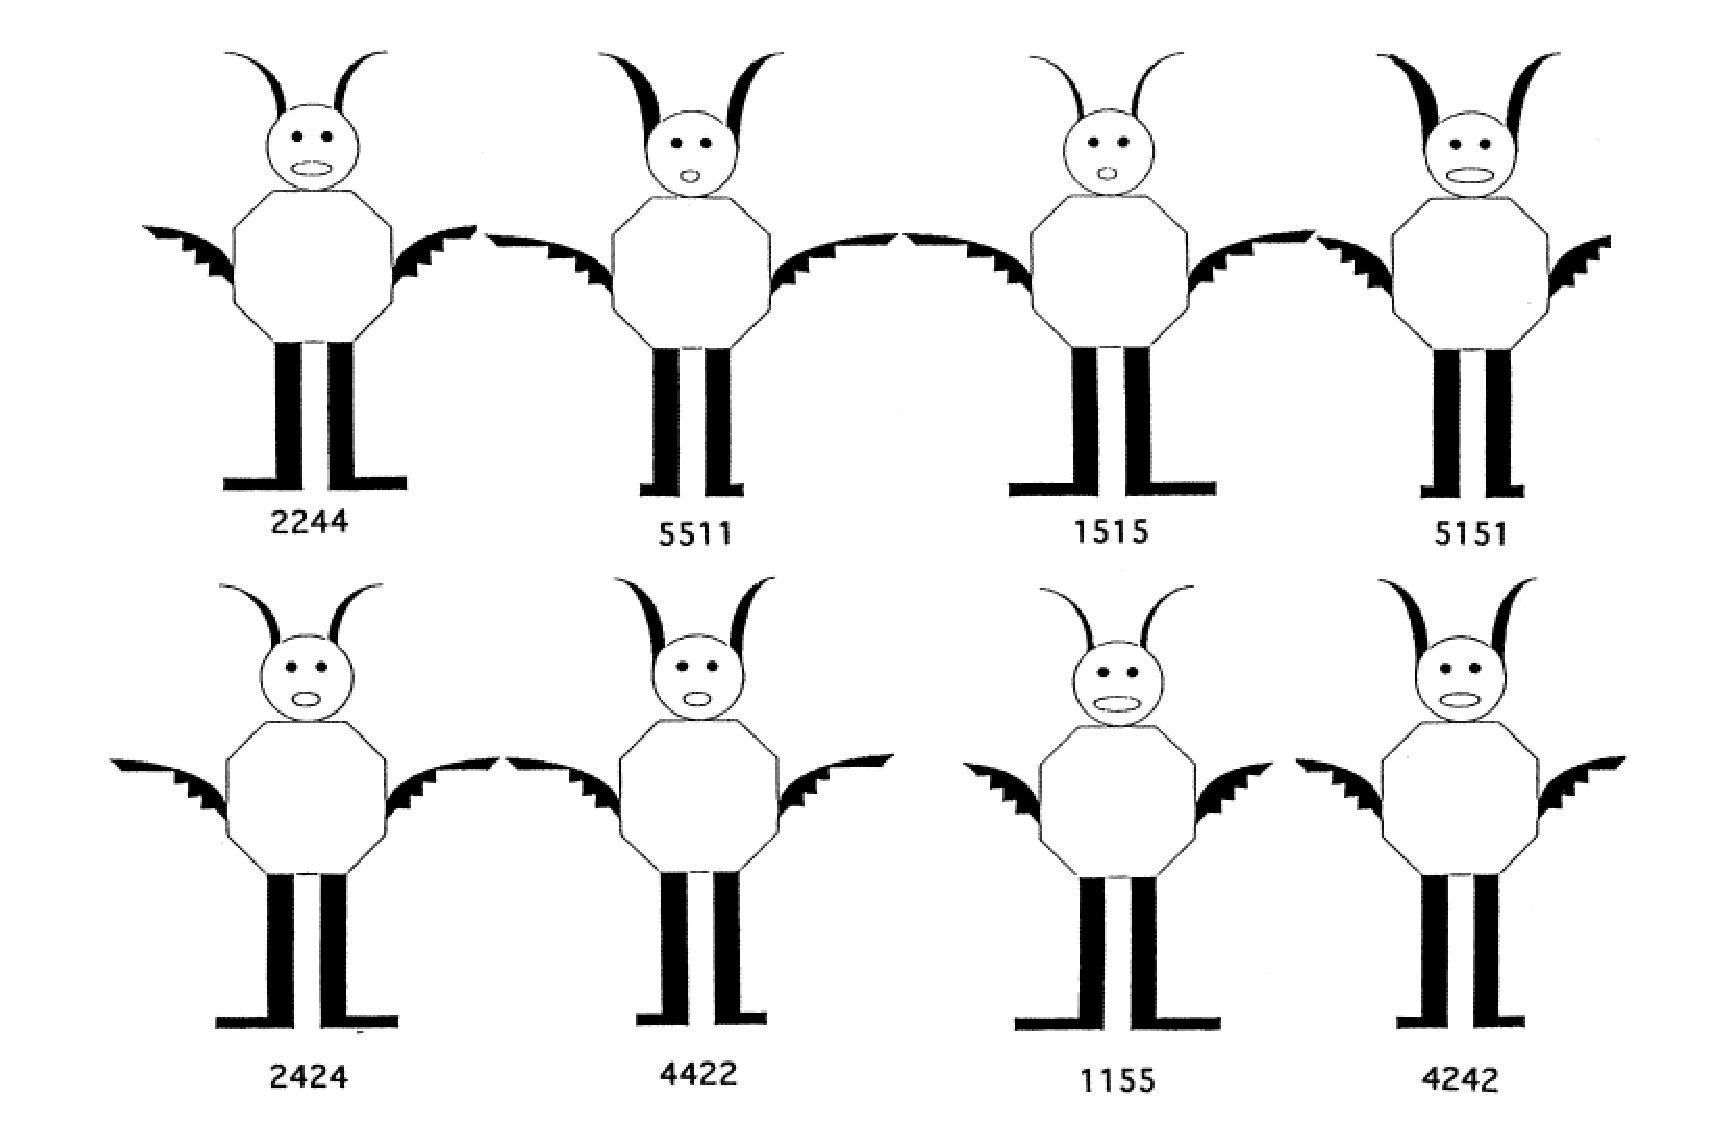
\includegraphics[width=75mm]{figures/mip_familiarization.eps}
\end{center}
\caption{Variation Within a Category. Image adapted from Klinger \& Dawson (2001).}
\label{mip-familiarization}
\end{figure} 

% DCN: WE NEED TO RECREATE THIS FIGURE WITH ONLY THE PROTOTYPE RESULTS!
% WE CAN ALSO LEAVE OUT THE DOWN SYNDROME BAR. THIS LEAVES SUCH A SIMPLE
% FIGURE THAT WE MIGHT WANT TO ELIDE THE GRAPH AND JUST REPORT THE 54 AND
% 79 PERCENT VALUES. INDEED, THAT IS WHAT I HAVE DONE.
% \begin{figure}[ht]
% \begin{center}
% 	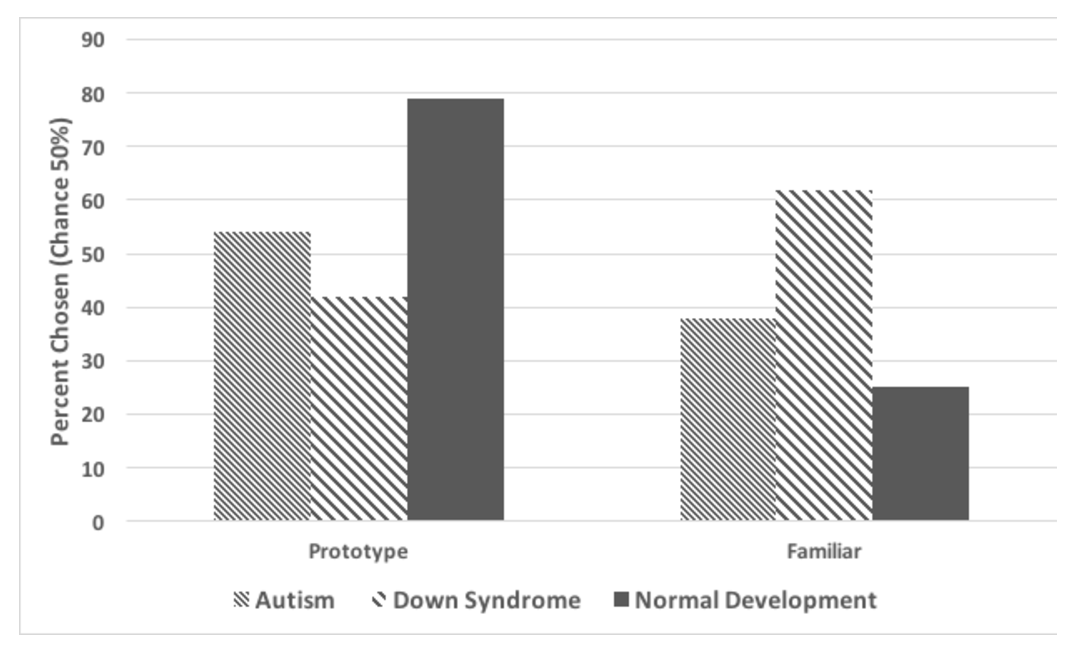
\includegraphics[width=110mm]{figures/klinger_results.eps}
% \end{center}
% \caption{Prototype Formation Results. The vertical axis shows the frequency with which the prototype was chosen over either a familiar or novel stimulus from the same category. Graph adapted from Klinger and Dawson (2001).}
% \label{klinger_results}
% \end{figure} 

\subsection{Modeling Category Learning with ALCOVE}
ALCOVE is a highly successful computational model of human performance on category learning tasks~\cite{KruschkeJK:1992:ALCOVE}. ALCOVE learns to categorize stimuli from corrective feedback on practice trials. There are three main processing layers in ALCOVE. An input layer represents the features of a current stimulus object. A hidden layer contains exponentially decaying radial basis function units, each of which becoming active to the degree that the current input is similar to that unit's preferred stimulus. The output layer contains one unit per category, with activation calculated as a weighted sum of hidden unit activity. The output activation levels are transformed into a probability distribution over category choices using a Luce choice ratio~\cite{LuceRD:1963:Ratio}. Learning arises from the adjustment of connection weights so as to reduce error~\cite{KruschkeJK:1992:ALCOVE}.

Importantly, ALCOVE also learns a set of attentional ``weights'' that reflect the relative importance of the various stimulus features for producing accurate categorization decisions. There is one weight value per stimulus feature (or ``dimension''), constrained to be between 0 and 1, with larger values indicating more sensitivity to variation in the given feature. ALCOVE's attentional weights determine the relative focus of the model on specific aspects of the stimulus, and are, therefore, analogous to the hypothesized role of PFC in directing top-down attentional control. (Consider the role of PFC in the previously described XT account of Stroop and WCST performance, focusing processing on specific aspects of the stimulus.) In the ALCOVE framework, PFC perseveration would involve restricting the attentional weights, limiting focus to one or a small number of the stimulus features.  

\begin{figure}[ht]
\begin{center}
	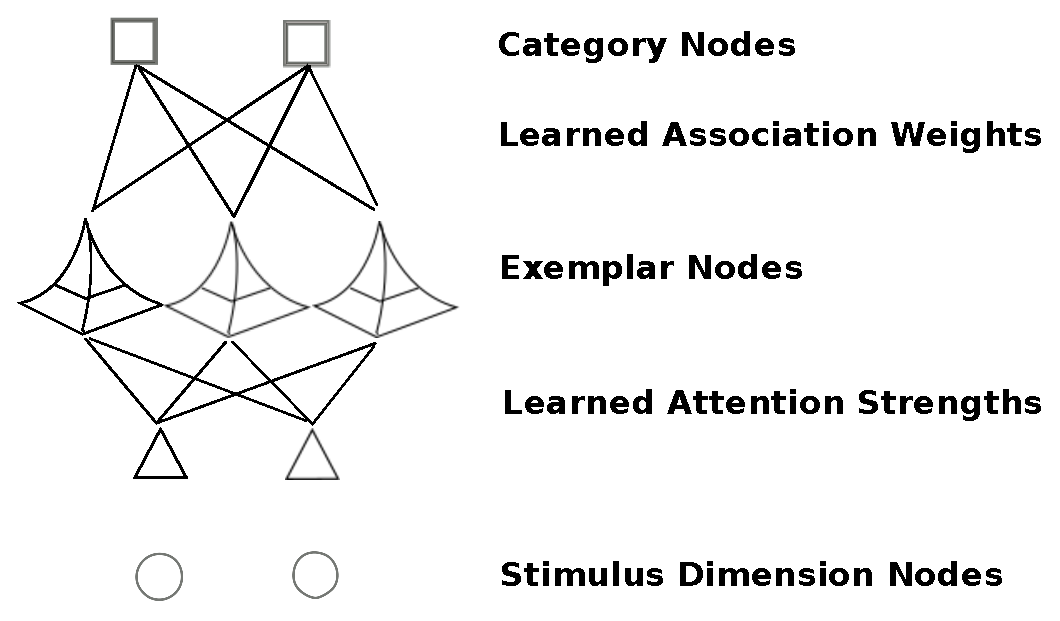
\includegraphics[width=75mm]{figures/alcove.eps}
\end{center}
\caption{Structure of ALCOVE (Attention Learning CoVEring map). Image adapted from Kruschke (1992).}
\label{alcove}
\end{figure} 

\subsection{Prototype Learning in ALCOVE}
We used ALCOVE to model the prototype formation study of Klinger \& Dawson (2001). Two output category units were used (e.g., ``Mip'' \& ``Non-Mip''). Four inputs, each with its own attentional weight, captured the four features that varied across members of the target category, with the 1--5 feature levels linearly scaled to 0.2--1.0 activations. (An activation of 0.0 was used to indicate the absence of a feature.) The model learned the target category from the same stimuli that were presented to children in Klinger \& Dawson (2001), with the standard ALCOVE error correction learning mechanism used to determine attentional and connection weights. Learning was disabled during subsequent testing for prototype formation.

% The training and testing of ALCOVE was modeled after the Klinger et al. study described above.  The training corpus was based on examples identical, in principal, to the target categories used during the familiarization trials. (See Figure~\ref{mip-familiarization}.)  As in the original study, eight familiarization trials were presented to the network during training.  On each presentation, the model labeled each target stimulus (e.g. this is a ``Mip'').  Only two response units, ``Mip'' \& ``Non-Mip'', were required.  Four input units, each with dimensional attention weights, were activated for each example presented to the network.  The four input units represent the four features used within each category in the study.  The level of activation for each input varied in a systematic fashion in accordance with the feature value of the stimulus.  For instance, if the stimuli presented has feature values (1551), the input vector presented to the network used the values (.20 1.0 1.0 .20). The standard ALCOVE error correction weight adjustments were used during the entirety of training.   After training ALCOVE on the familiarization stimuli, testing proceeded with all learning disabled in the model.  

Testing involved presenting the trained model with certain key stimulus objects and recording the activation of the target category output unit for each of them. The stimuli of interest included the prototype (``3333''), a stimulus seen during training (e.g., ``1515''), and a novel stimulus (e.g., ``1551''). For each pair of the prototype and another stimulus object, the recorded output activations were transformed into selection probabilities using a Luce choice ratio~\cite{LuceRD:1963:Ratio}. The mean probability of selecting the prototype over non-prototype stimuli was the measure compared to available experimental results.

% During testing, the prototype (3333) and the non-prototype test items, a novel stimuli (e.g. 1551) and a previously seen familiarization stimuli (e.g. 1515), were presented to ALCOVE separately.  The overall activation level of the output unit for the target category was recorded and used to determine which stimuli type was the ``preferred'' category example for ALCOVE. In order to compare model preference between prototype and non-prototype stimuli the activation levels were scaled to response probabilities using a Luce Choice Rule.   The average response probability for prototype versus non-prototype stimuli is the measure used in the comparison to the actual experiment results. 

\subsection{Modeling Autism in ALCOVE}
The ALCOVE model was modified in two ways to simulate neural differences in autism. First, we biased one randomly selected attentional weight to be high by initializing its value to $0.9$. The other attentional weights were initialized to $0.1$. This manipulation captures, at a gross level, our conjecture that deficient DA based gating of PFC results in overly perseverative control over top-down attention, effectively restricting the features used during processing. In the control version of the model, the attentional weights were all initialized to $0.1$, as is standard in ALCOVE. Attentional weights were adjusted during the category learning process, using the standard ALCOVE method for doing so. The second modification reflected the claim that ASD involves hyper-specific perception and behavior~\cite{HappeF:1999:WCC}. The ALCOVE ``specificity'' parameter, which controls the rate of exponential decay in the activation function of the hidden units, was increased from its standard value of $1.0$ to $2.5$ in the autism model. This caused each hidden unit in the autism model to become strongly active for a more restricted range of stimuli.

%One additional ALCOVE parameter was adjusted in order to better simulate the performance of people with autism on the categorization task.  The standard ALCOVE equation for the activation levels of the exponentially decaying hidden units contains a multiplicative scaling parameter referred to  by Kruschke as ``specificity''.  Increasing the specificity parameter makes the hidden units hyper-specific, sensitive to a more-restrictive range of features in the environment.  This is interesting because many researchers have argued that people with autism exhibit hyper-specific behavior in their everyday lives~~\cite{McClellandJL:2000:Autism,HappeF:1999:WCC}.  In the results described next, the specificity parameter in ALCOVE was adjusted from 1.0 in the control network to 2.5 for the network modeling behavior of people with ASD.  

%The simulated performance of people with autism will be contrasted with the control case, believed to capture normally developing people's performance on such tasks.  The performance of both autistic and control ALCOVE models will be directly compared to the data collected by Klinger and Dawson (2001). 

\subsection{Simulation Results}
Model simulations were repeated $80$ times in each experimental condition, with each repetition treated as an individual subject for data analysis. The control network exhibited the ``prototype effect'' observed in typically developing children, choosing the prototype over the non-prototype $70.52\%$ of the time.
% (See Figure~\ref{alcove-results}.)
For consistency, we used the same analysis as Klinger \& Dawson (2001), a one-sample T-test, in order to determine if the model's preference for the prototype was reliably different than chance (50\%). Analysis of the control model's performance indicated that the ``prototype effect'' was reliably larger than chance ($p < 0.0001$). The ASD model, however, preferred the prototype only $52.91\%$ of the time, which was not reliably different than chance ($p > 0.30$). This matches the lack of a ``prototype effect'' in people with autism reported in previous studies~\cite{KlingerLG:2001:Prototype,GastgebHZ:2009:Prototype}.

% DCN: Once again, it doesn't seem to make sense to have a figure for
% the display of only two values, given our space constraints.
% \begin{figure}[ht]
% \begin{center}
% 	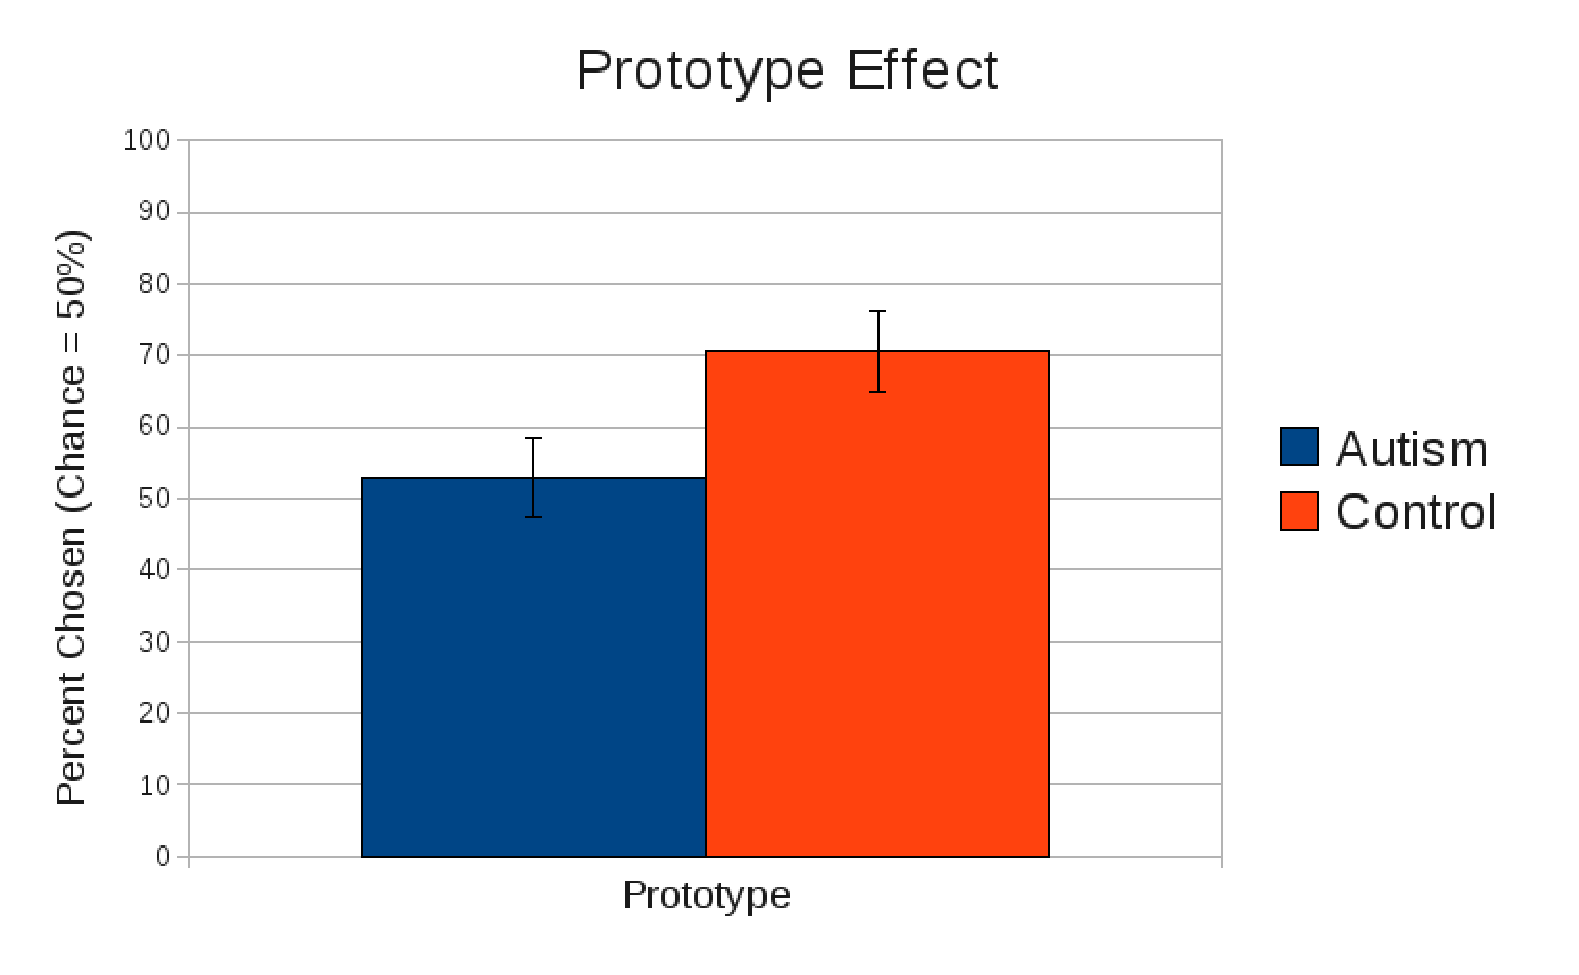
\includegraphics[width=100mm]{graphs/alcove_results.eps}
% \end{center}
% \caption{ALCOVE Model Results.  The measure on the y-axis is the percentage times that the prototypical animal was chosen by the model over the non-prototype choices.  In the control network, the prototype was chosen 70.52\% of the time on average, demonstrating a strong prototype effect and matching the human subject experiment results.  However, the model of autistic performance chose the prototype on average only 52.91\% of the time over the non-prototype stimuli.  Statistical analysis reveal that the control network chose the prototype at a rate significantly greater than chance ($p < .0001$) while the ASD network was not statistically distinguishable from chance ($p > .30$).}
% \label{alcove-results}
% \end{figure} 

\subsection{Summary}
These results show that failures at prototype formation in autism can be explained in terms of our hypothesized DA/PFC deficit. Restricting ALCOVE's attentional mechanism to hinder the flexible consideration of all stimulus features results in a lack of prototype preference. It is worth noting that matching the specificity parameter of the control model to match that of the autism model ($2.5$) does not change the presented pattern of results. This is evidence that it was the adjustment of initial attentional weights in the autism model, reflecting perseveration in PFC guided attention, that drove the observed difference.

